%\pagestyle{article}
\documentclass[a4paper]{article}
\usepackage[english]{babel}
\usepackage[utf8]{inputenc}
\usepackage{graphicx} % for figures
\usepackage[section]{placeins} %This prevents placing floats before a section.
\usepackage{csquotes}

\usepackage{wrapfig} % curtesy of LAURA PETRA - til dit billede i CV

% \usepackage{marginnote} % For margin years CV
% \newcommand{\years}[1]{\marginnote{\scriptsize #1}} % New command for including margin years
% \renewcommand*{\raggedleftmarginnote}{}
% \setlength{\marginparsep}{7pt} % Slightly increase the distance of the margin years from the contant
% \reversemarginpar

\usepackage{natbib}% better citation
%\usepackage{hyperref} %autoref
\usepackage[hidelinks]{hyperref} %hidelinks to remove ugly blue format
\usepackage{amsmath} % for \tag and \eqref macros in mathematical eq.

%% Sets linestretch, paragraphstrech, indentation and footnote stuff 
\usepackage{parskip} %space between paragraphs
\parskip=12pt %set space between paragraphs
\setlength\parindent{12pt} %paragraf indentation
% \usepackage[onehalfspacing]{setspace} %linespacing; does not affect footnotes
\usepackage[doublespacing]{setspace} %linespacing; does not affect footnotes

\setlength{\footnotesep}{0.7\baselineskip}% space between footnotes
\usepackage[hang,flushmargin]{footmisc} %% removes identation in footnoteshttps://www.overleaf.com/project/5b98e00a21d3bd15ac5a2e86

\usepackage{makecell} % make cells in tabels for longer text

\usepackage[colorinlistoftodos]{todonotes}

%% For header and footer (1)
% Marco
\usepackage{fancyhdr}
\pagestyle{fancy}
\textwidth = 452pt% 424pt % test width ish
\oddsidemargin = 0pt %18pt % margin width ish

\fancyheadoffset{0 in} % Shifty solutions..

\fancyhf{} %% clear defuelt header and footer

%% For header and footer (2)
%Specifics
\lhead{Maase \& Spanner}
\rhead{\today}

\lfoot{University of Copenhagen}
\rfoot{\thepage}
\renewcommand{\footrulewidth}{0.8pt}

\title{\textbf{Bodies as Battleground} \\ Sub-project 2}

\author{Simon Polichinel von der Maase \\ \& \\ Johan Spanner}
\date{October 2019}

\begin{document}

	\begin{titlepage}
		\maketitle
		%Character count: 43.950/44.000\\
		\noindent\rule{\linewidth}{0.4pt}
		\begin{figure}[h]
			\centering
			
\includegraphics[scale=0.32]{KU_logo.png}
		\end{figure}
		\thispagestyle{empty} % removes page number on front page
	\end{titlepage}
    \tableofcontents
\pagebreak

% \section{Application} if below should be subsections.

\section{Presentation}

% What is sub project 2?
The fundamental question of sub-project 2 is whether there is: \textbf{" a correlation between the level of violence in armed conflict and the representation of gender in war photography?"}. As such, "[t]his research project asks how gender norms are expressed -- or not -- in photographs during armed conflict.". The theoretical expectation is that: "as levels of violent conflict increase, there is frequently a turn to more traditional gender norms". \par

% Regarding the hypothesis
Naturally we will need more concrete hypotheses regarding specifically how we except gender norms to correlate with the level of violence.
As presented in the original project description, we presently have six hypotheses:\par

\begin{description}

    \item[H1]: as the level of violence increases, there will be fewer images of women in public spaces.
    %(Should be ratio to men (in public spaces?)... or?.. But what about the well and the marketplace?)
    
    \item[H2]: as the level of violence increases, women will be photographed in more conservative clothing.
    %(Should be ratio of women in religious (traditional?) clothing - or?)

    \item[H3]: as the level of violence increase, we see an increase of images featuring men in the role of protectors. 
    %(... More male soldiers compared to female soldiers???)

    \item[H4]: as the level of violence increase, there is an increase of images featuring women as in need of male protection. 
    %(More pictures of female citizens with foreign (male) soldiers )
    
    \item[H5]: as levels of violence increase, there is an increase of images showing women responding emotionally.
    %(crying? screaming? Preying? Kneeling?)

    \item[H6]: as levels of violence increase, there is an increase of images showing men acting with reason and restraint.
    %(Assisting someone? Talking? Looking stoic????)

\end{description} \hfill \hfill ...

% Conditional hypotheses:
Beyond this, we are also interested in illuminating whether the gender of the photographer makes a difference and whether there is a difference between the gender norms presented in the raw shoots, the pictures sent to the editor, and the pictures published.\par

% bridge
We shall return to the hypotheses later and the possibility of qualifying the ones presented as well as formulating novel additions. For now, however, the hypothesis presented simply serve as context, illustrating the kind of information we need our data to capture.\par

\section{From pictures to dataset(s)}
% The Data from Uppsala
First of all, a very brief introduction of the conflict event dataset from Uppsala (UCDP) is in order. To operationalize the measure "level of violence" denoted in the hypotheses above, we will use the \textit{UCDP Georeferenced Event Dataset (GED) Global version 19.1}\cite{Sundberg_2013}. Given our project, the most relevant feature in this dataset are the four pertaining to; conflict fatalities, date, latitude and longitude. With this information we will know (approximately) how many people died when and where during the conflicts covered by the photographers. This is how we shall measure "the level of violence". As such, these features will be matched with our own data.\par 

% From master thesis:
%I define conict fatalities using the minimal definition from UCDP. They include in their data all fatalities where "[...] armed force was used by an organized actor against another organized actor, or against civilians, resulting in at least 1 direct death at a specific location and a specific date" (Croicu and Sundberg, 2017, 9).

% Our own data

% the two different datasets we produce
To give you an understanding of what our own data actually is -- or will be -- I will need to describe two different datasets. I do this since the first dataset serves as basis for the second. The first dataset takes the individual picture as the unit of analysis. The second takes some temporal/spatial aggregation as unit of analysis. The second dataset will be the dataset which we merge with the data from Uppsala and ultimately use to test our hypotheses. The dataset taking the images as unit of analysis will be called the "image dataset" while the second dataset will be called the "aggregated dataset". Creating the image dataset will be our point of departure. For each image in this dataset we will have information regarding the time, date and location of that image, the name of the photographer along a number of features denoting what we see in the image. E.g. number of humans, number of men, number of women, number of women with religious garments, whether women in the image is portrayed as in need of male protection etc.. Before we can merge this data with the conflict data from Uppsala we will need to aggregate the data at some suitable temporal and spatial unit of analysis appropriate for our hypotheses. This is where we create the second aggregated dataset. Each entry in this second dataset will be some geographic location at some time period. Say, Baghdad, January, 2005. Beyond the specific information regarding time and place, the features in this dataset will be composed of the aggregated information from all images taken at the specific location during the specific time frame. E.g. total number of males in all images taken in Baghdad, January, 2005; Total number of females in all images taken in Baghdad, January, 2005 etc.. Information which can naturally be transformed into ratios and so on given the need. \autoref{imgset} illustrates the structure of the image dataset while \autoref{aggset} illustrates the structure of the aggregated dataset.\par

%What do we want the image dataset to look like:
\begin{table}[ht]
\caption{Likely structure of image dataset (when done)}\label{imgset}
    \begin{tabular}{|*{9}{p{1.32cm}|}}

        \hline
        \multicolumn{9}{|p{15.4cm}|}{Image dataset} \\ % should you just have a title?
        \hline  image* & date & time & location & author & $x_1$ & $x_2$ & $\dots$ & $x_n$ \\
        \hline
        $i_1$ & $d_1$  & $t_1$  & $l_1$  & $a_1$  & $x_{11}$  & $x_{21}$  & $\dots$   & $x_{n1}$  \\
        $i_2$ & $d_2$  & $t_2$  & $l_2$  & $a_2$  & $x_{12}$  & $x_{22}$  & $\dots$   & $x_{n2}$  \\
        $i_3$ & $d_3$  & $t_3$  & $l_3$  & $a_3$  & $x_{13}$  & $x_{23}$  & $\dots$   & $x_{n3}$  \\
        $\vdots$ & $\vdots$  & $\vdots$  & $\vdots$  & $\vdots$  & $\vdots$  & $\vdots$  & $\vdots$   & $\vdots$  \\
        $i_n$ & $d_n$  & $t_n$  & $l_n$  & $a_n$  & $x_{1n}$  & $x_{2n}$  & $\dots$   & $x_{nn}$  \\
        \hline
    \end{tabular}
    
    {\raggedright \footnotesize{*At some point in the process this will be the actual image, but later on it will simply be some id referring to the specific image} \par}
    
\end{table}

%what do we want the aggregated dataset to look like:
\begin{table}[ht]
\caption{Possible structure of aggregated dataset (when done)}\label{aggset}
    \begin{tabular}{|*{9}{p{1.32cm}|}}%\label{imgset}

        \hline
        \multicolumn{9}{|p{15.4cm}|}{Aggregated dataset} \\ % should you just have a title?
        \hline  city* & week** & month & year & deaths*** & $\chi_1$**** & $\chi_2$ & $\dots$ & $\chi_n$ \\
        \hline
        $c_1$ & $w_1$ & $m_1$ & $y_1$ & $d_1$ & $\chi_{11}$  & $\chi_{21}$  & $\dots$   & $\chi_{n1}$  \\
        $c_2$ & $w_2$ & $m_2$ & $y_2$ & $d_2$ & $\chi_{12}$  & $\chi_{22}$  & $\dots$   & $\chi_{n2}$  \\
        $c_3$ & $w_3$ & $m_3$ & $y_3$ & $d_3$ & $\chi_{13}$  & $\chi_{23}$  & $\dots$   & $\chi_{n3}$  \\
        $\vdots$ & $\vdots$ & $\vdots$ & $\vdots$ & $\vdots$ & $\vdots$ & $\vdots$  & $\vdots$   & $\vdots$  \\
        $c_n$ & $w_n$ & $m_n$ & $y_n$ & $d_n$ & $\chi_{1n}$  & $\chi_{2n}$  & $\dots$   & $\chi_{nn}$  \\
        \hline
    \end{tabular}
    
    {\raggedright \footnotesize{* city will probably not be the spatial unit of analysis. Instead we might use what is called \textit{PRIO grid cells}, but for simplicity \textit{city} will do for now.} \par
    \footnotesize{** the "smallest" temporal dimension has not been decided on, but weeks or months will do fine.} \par
    \footnotesize{*** From the UCDP. We will most likely be using the log of conflict fatalities, but this is not important at this point.} \par
    \footnotesize{**** $\chi_i$ here used to denote that we have aggregated the features $x_i$ at some temporal and spatial level - in this example city and week.}
     \par}
     
    %  \footnotesize{*** $\Sigma$ here simply denoting that it is the sum of $x_i$ of all images taken doing the "smallest" temporal dimension used.}
    
\end{table}

% comments on the tables?
% ... something from the notes?

% bridge
The $x_i$'s in the image dataset are here placeholders for the actual features pertaining to the hypothesis; that is information regarding what is \emph{in} the specific image. There are two ways to get this information. Manual labeling for each image according to some preconstructed code-book and automated object recognition via machine learning. We will use both approaches in tandem, both will be introduced below as will the manner in which they support each other.\par

%HOV! du nævner nogle andre x her under; dem fra image set.. Det skal du lige søger for ikke forvirrer folk... Er det ikke i vikeligheden y'er i tabellen.??

\subsection{Automatic classification}
% What is this shit? 
% Fra Johan: nederste linje i para - mener du a light introduction? -> fra Simon: nope. Light intuition.. Men light introduction er også fint..
In recent years we have seen a huge improvement in the ability of machine learning algorithms to identify and classify objects in images. This improvement is largely due to developments within the field of deep learning, specifically the development of \emph{Convoluted Neural Networks}  \citep[120-122]{francois2017deep}. Now, I shall not bore you needlessly with technicalities, but some light intuition will be of service.\par

% a linear regression:
Imagine a simple linear regression, we could use this as a linear probability model to determine whether some creature is a dog or a cat. In this example we do not use the pictures yet. Instead we have data on four features pertaining to a number of cats and dogs. E.g. "snout to face ratio", "shape of legs", "ear placement" and "general smugness". Using the magic of math we now estimate the most likely relationship between our input data -- the features ($x_i$) -- and our output data -- the \emph{target} ($y_i$). Our linear probability model would appear as presented in \autoref{linMdl}.\par

\begin{figure}[!htb]
	\centering
	\caption{linear Model}\label{linMdl}
	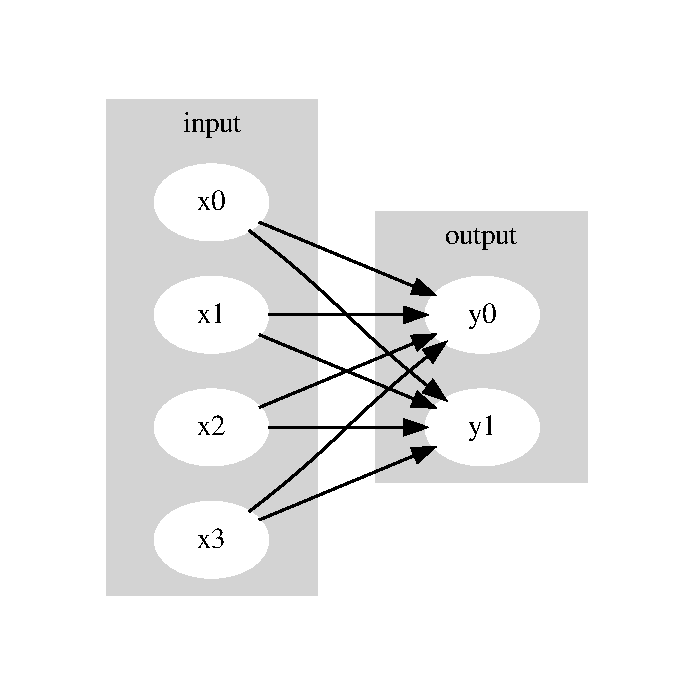
\includegraphics[scale=0.55]{linMdl.pdf}
\end{figure}

% What happens in the linmdl.
Here we know the features of the creatures (the input) and whether they are a cat or a dog (the output). The output is our target and the linear probability model allow us the estimate the probability between e.g. a creature looking very smug and being a cat. The arrows in \autoref{linMdl} here holds these estimated probabilities. Importantly once the model is trained on data containing both features and target -- that is, the values of the arrows have been estimated --  we can introduce new data where we only have information pertaining to the features. As such, we can ask our model to classify new creatures for which we do not know the species (cat/dog) but do know the features. This is called \emph{out-of-sample-prediction} and it is naturally out-of-sample prediction which will allow us to automatically classify various elements of images, for which we do not yet know the content.\par

% a dense neural network
% FRa JOHAN forslag That is, we may believe that the relationship between our features might be more complex -- that there could be interactions or non-linear relationships.
Now, before we get ahead of ourselves we might argue that \autoref{linMdl} presents a model too simple to capture the subtleties between cats and dogs. That is, we may believe that the relationship between our features might be more complex -- that there could be interactions or non-linear relationships. We could try to model such a relationship manually but this can be both bothersome and inefficient. Instead lets simply use an algorithm which automatically identifies and generates relevant non-linearities itself. Artificial Neural Networks are such algorithms \cite{francois2017deep, williams2019images}. A rather simple three layers deep neural network is presented in \autoref{annMdl}.\par

\begin{figure}[!htb]
	\centering
	\caption{Artificial Neural Network}\label{annMdl}
	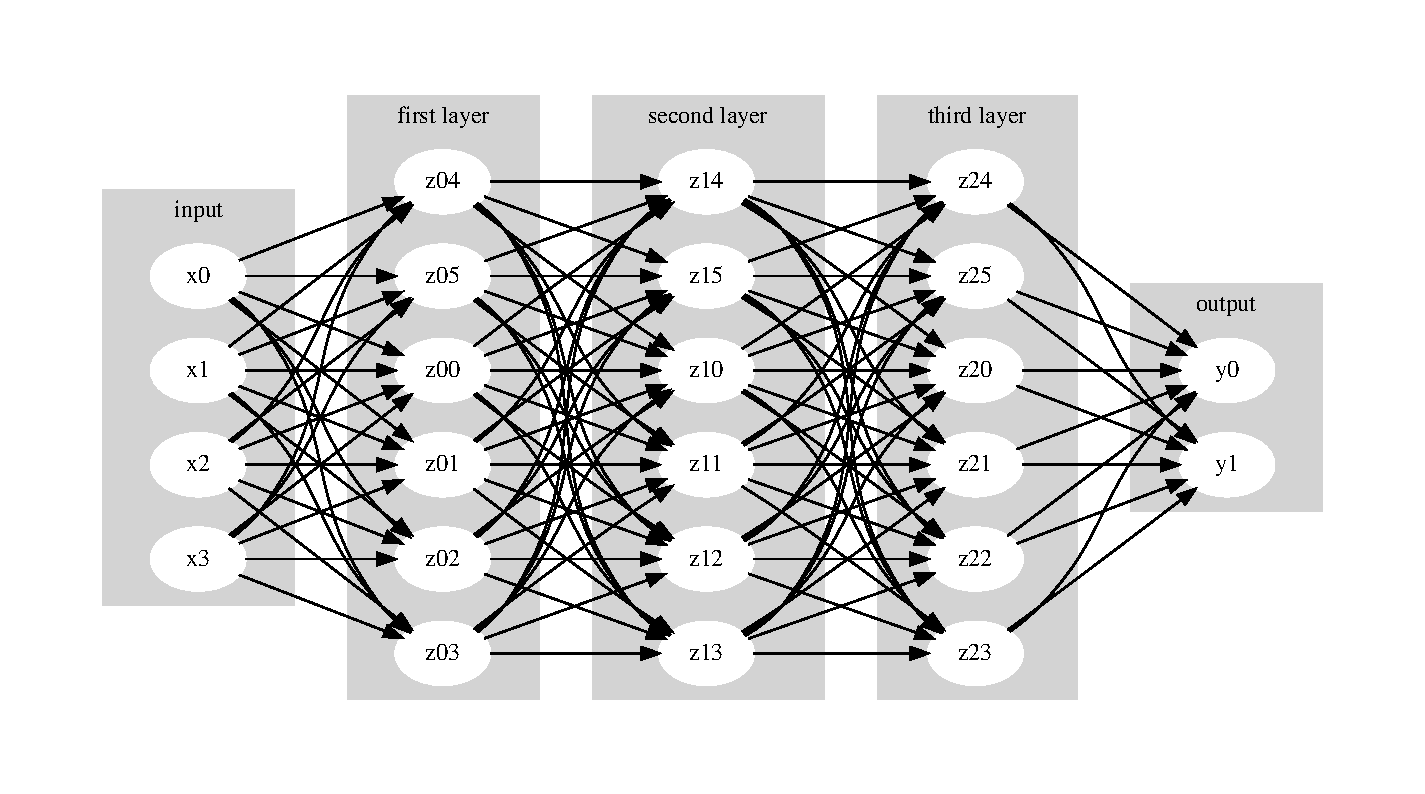
\includegraphics[scale=0.65]{annMdl.pdf}
\end{figure}

% why is this different?
The difference here is that we now have a number of \emph{layers} between our input and output data. In this case we have three layers, each containing six \emph{nodes} ($z_{ji}$). In reality most artificial neural networks have far more nodes, layers of various sizes and a lot of other complexities which we shall not go into here. It is these layers and nodes which allow the network to automatically identify and generate relevant interactions and non-linearities. Here a specific "snout to face ratio" combined with a specific "ear placement" might equal "cat" if "general smugness" is sufficiently high. Given the complexity of such Neural Networks they are harder to interpret than methods such as linear regressions, but in return they are often much more capable of making accurate predictions - especially \emph{out-of-sample} \cite{williams2019images}.

% out of sample -> pictures
Making predictions out-of-sample is exactly what we want to do here. We want to predict what is \emph{in} pictures -- pictures which were not a part of the sample we use to train our model. Now, to classify images we will use what is called a Convoluted Neural Network. I will not go into the architecture of such networks here since it is, well, convoluted. But the intuition is the same as with the network presented in \autoref{annMdl}. Instead of some features, imagine that we feed it digital image data directly: simply the pixels of the image. Each consecutive layer will learn different shapes relevant related to the target of interest. The deeper we go the more complex the shapes get. The first layers might identify lines or edges, then triangles and squares might be captured by later layers and as we go deeper; circles, eyes, faces, people and so on depending on what the targets in the output layer are.\par % du skal have skrevet mere om target tidligere...

% we could train our own network, but there are very good of the shelf available
For our project we could construct our own network from scratch, but this usually requires millions of pre-labeled images. Thus such endeavour appears quite unfeasible. First of all we might not have enough images in our whole dataset to train a good network. Secondly, it would be quite a burden on our student assistants; demanding of them to label millions of pictures (in which case the need for automatic classification would also vanish). Encouragingly a number of \emph{pre-trained} models such as ResNet are in existence, and are trained to capture thousands of different categories \cite{williams2019images}. The extent to which such networks hold the categories we need is not yet clear, but they will hold many relevant generic categories such as "human", "male", "female" and so on.\par

% our own cats.
However, we should not expect more specific categories relating to our hypothesis to be included in the pre-trained networks, e.g. whether a women is dressed in traditional/religious garment. Luckily there is a convenient solution here. Since the pre-trained networks have already learned the most fundamentally interesting shapes for any or most classifications tasks in the early and mid-level layers, we can simply insert our own manually labeled output data as target and retrain the last layer or couple of layers. This is called \emph{transfer learning}, because we transfer information obtained from one prediction task to help with a different prediction task \cite{williams2019images}. It has been showed that such \emph{fine-tuning} of pre-trained networks can yield very accurate results even with relatively little new data, say a 100 to 1000 new images \cite{williams2019images}. As such we can fine-tune such pre-trained models to capture very specific categories while still keeping the resource devoted to manual labeling to a minimum (and saving our student assistants from a very tedious work load...).\par

% summarize and bridge:
Using pre-trained networks and fine tuning based on our own labeled data we should be able to impute all features of interest and attach this information to each of our images in the image dataset. These features will then be aggregated at some appropriate temporal and spatial level for the aggregated dataset which will then be merged with the relevant data from Uppsala. This is how we turn images into data appropriate for our project. First, however, there is still the matter of manual labeling.\par

\subsection{Manual Labeling}

% So, what exactly is this all about?
While pre-trained networks will help us a lot, some manual labeling is inevitable. Given our project, we will be interested in a lot of very specific features which are surely not captured by the pre-trained models; whether women wear conservative/religious garments, whether the picture features women as in need of male protection, whether the images shows women responding emotionally etc. In order to capture such specific features we will need to manually label a sample of our images ourselves. This sample will then be used to fine-tune the pre-trained networks.\par

% how:
This manual labeling is straight-forward. The student assistants -- and possibly me - simply look at the pictures and document whether a relevant feature is present in the image or not. Naturally the decision regarding whether or not some feature is present in some image will not be ad hoc. We will follow a elaborate yet concise codebook describing exactly what we mean by e.g. "conservative garments". It is also possible that such elements are best captured by more features. E.g. that we should distinguish between different kinds of conservative and religious garments. Likewise "in need of male protection" could mean many things and thus we should capture such elements with a roster of more concrete features. This will allow for deeper analysis later on, it will help us produce more fine-grained conclusions and it will lessen any ambiguity of the manual labeling process.\par

% creating such codebook
As with the creation of any codebook -- be it for manual labeling, interviews or similar -- the process of creating it will begin with our theory and hypothesis. Then there will be an iterative process where we go forth and back between small random samples of images and theory until we are confident that the codebook can serve to link theory with the content of the images. Once we are satisfied with the codebook we will start labeling a large, random, sample of the images. It is this sample we will use to fine-tune the pre-trained model(s).\par 

% inter-coder reliability - we code the same images.
While a well-constructed codebook should ensure reliability in the labeling effort, we can not trust it blindly. As such, the coders -- potentially the two student assistants and myself -- should ideally label the same roster of images or at least an overlapping subset allowing us to test the inter-coder reliability and to assess any ambiguity in the labeling process. That is; assessing whether, and to what extent, all coders agree upon what the various images actually depicts. Were all three coders to label the same complete set of images, we would be able to asses, discuss, handle or potentially drop images where the labeling exhibited discrepancy. If only a subset of the coded images are labeled by all coders handling becomes more problematic, but at least we can still assess and report how well our labeling matched, using some measurement for inter-coder reliability such as Krippendorffs alpha or similar. 

% How many?
Naturally this raises the question of how many images to hand-label. As mentioned, it has been found that 100 to 1000 new images can be enough to achieve rather high accuracy on novel categories using a fine-tuned pre-trained model. However, it should here be noted that this is 100 to 1000 images pertaining to one new category in a balanced dataset. As such if I were to use a pre-trained model to classify dogs from cats I would need 50-500 images of cats and dogs respectively. Point being, it is not enough to simply label 100 to 1000 completely random images from our dataset. Instead we must label at least 50 -- and most likely many more -- images containing the element of interest for each category which we want to capture and likewise at least 50 images \emph{not} containing the element(s) we want to capture. Furthermore, all or some of these images should be coded by more than simply one coder to asses and ensure prudent inter-coder reliability. Point being, at the time of writing we cannot say how many images will need to be hand-labeled. Disregarding how we decide to handle inter-coder reliability the amount of images to be hand labeled largely depends on the number and nature of the final hypotheses.\par

% Shortcut

% and something about accuracy.

% what categories?

% bridge to hypothesis:
The reason, naturally, is that the elements which we want to capture flow directly from the hypotheses formulated. This leads us to the next subject.\par % lame bridge.. 

\subsection{Hypotheses}

\begin{displayquote}
\emph{"A wise man ought always to follow the paths beaten by great men, and to imitate those who have been the best, so that if his ability does not equal theirs, at least it will have some traces of it.}

\emph{He should act like those who are skilled at shooting with a bow and arrow who, designing to hit the mark which yet appears too far distant, and knowing the limits to which the strength of their bow attains, take aim much higher than the mark. This is not done in order to reach a great height, but to be able with the aid of so high an aim to hit the mark they wish to reach."}\par

\hfill \hfill Machiavelli, the prince (1532), chapter 6 %, 1st paragraph
\end{displayquote}

% point with that quote
This quote (aptly extended to wise and great women as well) is a good starting point for our discussion regarding the hypotheses. Our hypotheses should spring from well founded theory and, as a starting point, we should strive to formulate hypotheses which actually describe the theoretical mechanisms proposed by the literature. Indeed we should try to capture what is often refereed to as \emph{the "true" data generating process} in all its unwieldy complexity. Later in the process we will be forced to make plenty of simplifying assumptions in order to emulate the hypotheses via quantitative models but a comprehensive starting point based on precise expectations will help us distill complex theory into concise hypotheses -- we aim high to strike true.\par

% Measurement
In practice, good theoretical foundations will also help us link the individually hypothesis to measurement and further to the construction of the codebook. Indeed we want to know exactly what we want to measure, even if the thing we want to measure is in essence unmeasurable. Knowing precisely what we want to measure qualifies us to create measurements when feasible, find proxies when possible and abandon hypotheses where no practical conceptualisations appear possible or prudent.\par
 
% All models are wrong...
Importantly, the fact that we must inevitably go from complex theory to simplified hypotheses should not discourage us. Using quantitative methods one can never capture the full complexity of the real world: "In the end all models are wrong, but some are useful" (proverb, usually contributed to the British statistician George E.P. Box, 1976). What we need is simply to make robust and transparent models which can help illuminate the research field of our project.\par

% Bridge
Formulating our roster of hypotheses is presently the prime challenge. We need the hypotheses before we can begin the constructions of the codebook and further the labeling of our images. However, while the construction of the hypotheses is the prime challenge -- and notably the challenge where your knowledge and expertise is most directly required -- there are a few other practical challenges which also needs attention. These are the challenges which Johan and myself have been working on the last couple of weeks and which mostly pertain to the practicalities of constructing the dataset(s). These challenges will be the subject of the next and final section and as such, said section should be seen simply as an update on the work current state of affairs.\par

\subsection{What we are doing right now} % comes rather late.. But that is ok. You start backwards (to some extent...).

% What we are doing right now.
...

% raw/edit/pupl.
The images can be understood as belonging to one of three \emph{bins}: Raw shoots, images sent to editor and published images (either on print or online). This is illustrated in \autoref{bins}. Going forth I will focus mostly on the bins "raw" and "edit".\par 

\begin{table}[ht]
\caption{Image "bins"}\label{bins}
\centering
    \begin{tabular}{|*{3}{p{4cm}|}}%\label{imgset}

        % \hline
        % \multicolumn{3}{|p{12cm}|}{Image "bins"} \\ % should you just have a title?
        \hline  raw & edit ($\subseteq$ raw, $m\leq n$) & published ($\subseteq$ edit, $k\leq m$) \\
        \hline
        $r_1$ & $e_1$ & $p_1$   \\
        $r_2$ & $e_2$ & $p_2$   \\
        $r_3$ & $e_3$ & $p_3$   \\
        $\vdots$ & $\vdots$ & $\vdots$   \\
        $r_n$ & $e_m$ & $p_k$  \\
        \hline
    \end{tabular}
    
\end{table}

% What, respectively, raw and edit holds
The images in the "raw" bin holds only the meta information provided by the camera used -- most crucial for our project is the time and date of image. Unfortunately the cameras used at the time of the conflicts did not automatically geotag the images, thus there is no information regarding location held in the metadata of the raw shoots. The images in the "edit" bin naturally have the same meta data on time and date as the raw shoots, but these images are also accompanied by more comprehensive meta data entered by the individual photographer. This meta data pertains to location, copyright, a short description of the captured scenario and more.\par 

% interpolating locations with machine learning
Naturally we need to figure out the location of the raw shoots if we are to combine our image data with the conflict data from UCDP. Encouragingly, given that the edited images are simply a subset of the raw images we can infer where the raw shoots were taken by comparing the time and date of the raw shoots with that of the edited images. Even more encouragingly this is easily automated using machine learning.\par

% Example
To exemplify let's look at a small subset of images taken on two different days across to different cities. In \autoref{editImg} we se how a very small sample of Johan's images are distributed across time, data and location. The first day all images were shot in the same city. The second day Johan started in the same city but changed location some time doing the day as seen by the color shift.\par


\begin{figure}[!htb]
	\centering
	\caption{Images from edit (with location)}\label{editImg}
	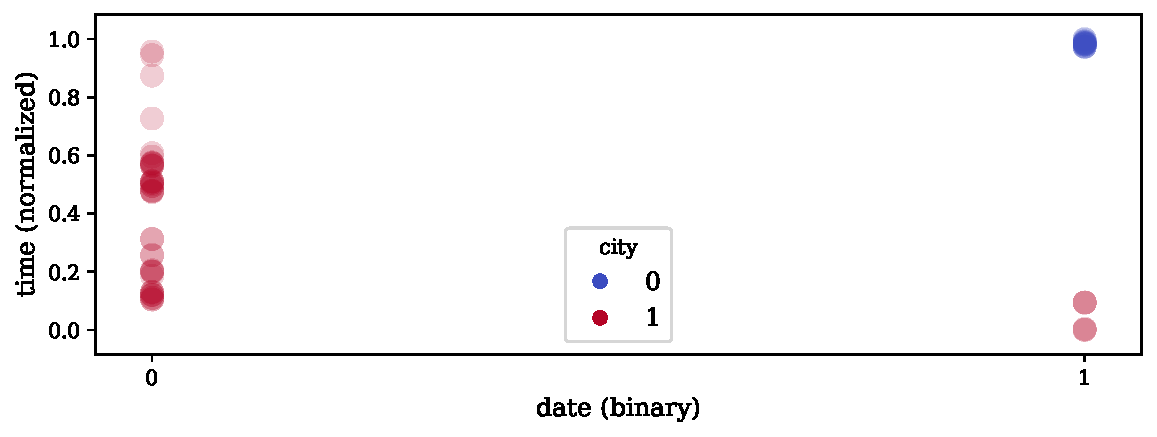
\includegraphics[scale=0.65]{edit_img.pdf}
\end{figure}

% trainig the model
Now we train some machine learning algorithm to recognize the pattern exhibited here. I use time and date as my two input features and city as my sole target. The specific algorithm here used is called Support Vector Machine (RBF kernel) which is well suited for such classification tasks. Here the task is binary -- I only have two cities -- but the method generalised neatly to task with many more targets. The result can been seen in \autoref{svmImg}.\par
 
\begin{figure}[!htb]
	\centering
	\caption{Creating Model with SVM}\label{svmImg}
	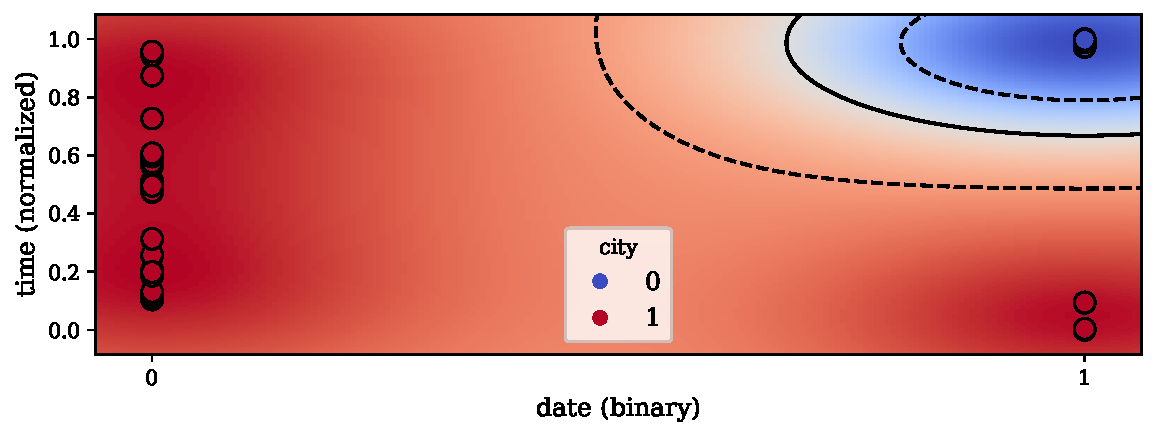
\includegraphics[scale=0.65]{svm_edit_img.pdf}
\end{figure}

% interpret plot above
The color gradient represent the probability of an image being from one of the two cities. The solid represents a hard threshold and the dashed lines the 95\% confidence interval of said threshold. This model can now be applied to classify images from the raw bin, where we do not have any prior information regarding location.\par

\autoref{rawImg} Show a sample of images from Johan's raw bin. We know he time and date of the images, but as indicated by the gray color of the points we do not know the location.\par

\begin{figure}[!htb]
	\centering
	\caption{Images from raw (without location)}\label{rawImg}
	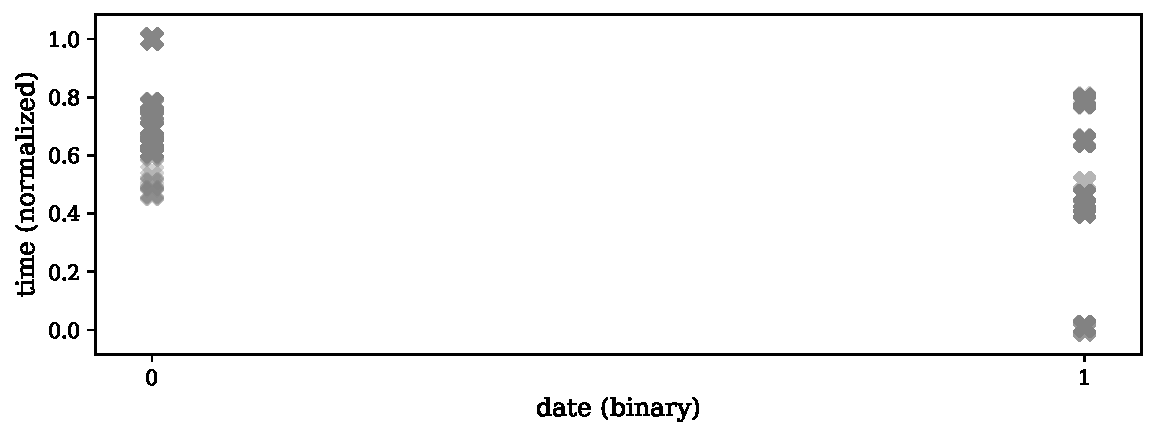
\includegraphics[scale=0.65]{raw_img.pdf}
\end{figure}

Using our model we can now classify these images as having originated in one of the two cities. This is shown in \autoref{predImg}. Here the images from edit are represented by dots while images from raw are represented by crosses. As seen all images are now classified according to our model.\par

\begin{figure}[!htb]
	\centering
	\caption{Applying model on new data}\label{predImg}
	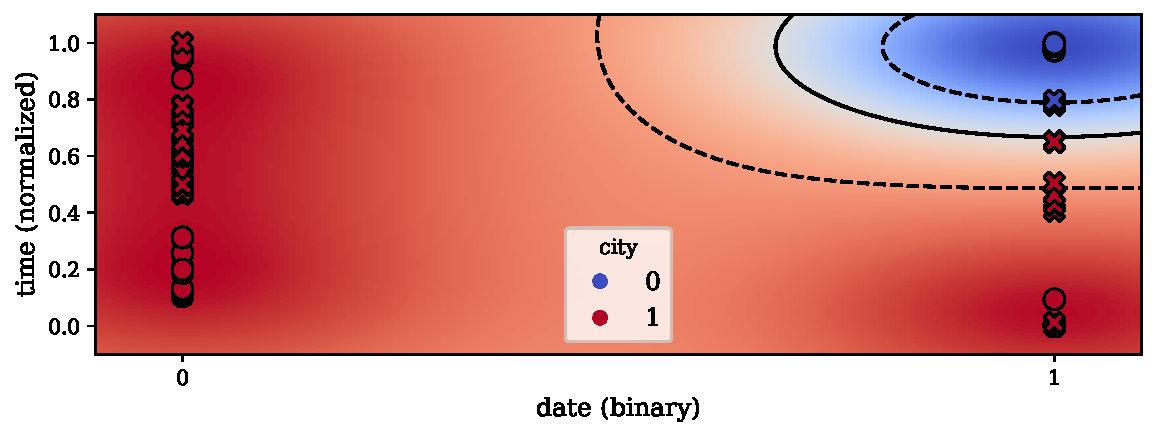
\includegraphics[scale=0.65]{pred_img.pdf}
\end{figure}

% dropping ambiguity
Notably however, some of the images from the raw bin are taken at times where our model has little to no information. To use these images would be imprudent. Luckily we can simply set some threshold -- say 90\% -- and demand that the probability of a given images belonging to one of the two cities should be above this threshold if the image are to be part of our final dataset. Notably the images in danger of being discarded by this sorting process will largely be images taken doing transportation and thus of limited interest to us. This also holds for raw images taken a given day before the first edit image and after the last edit image. As such we have also discussed dropping all images outside this span. It should also be noted, however, that using all images and not just a small sample will ensure less ambiguity then what is presented above.\par

This concludes the presentation on where we are and where we are going. Naturally a lot of subject matter was left out for the sake of brevity. This includes, but is not limited to, the challenge pertaining to the published images and indeed all and any discussion regarding the models which we will actually use to test our hypotheses. While important these subjects will be saved for later discussions, when the challenges most pressing right now have been adequately solved.\par

% Drop if you think it is to cheesy or to informal...
Best Regards\\
\emph{Johan Spanner \& Simon Polichinel von der Maase}

\pagebreak

%\section{References}
% - Temporary
\bibliographystyle{apalike} 
\bibliography{app_conf.bib} % what to use...

\end{document}
